%% 
%% Copyright 2007-2025 Elsevier Ltd
%% 
%% This file is part of the 'Elsarticle Bundle'.
%% ---------------------------------------------
%% 
%% Template article for Elsevier's document class `elsarticle'
%% with numbered style bibliographic references
%% Adapted for Knowledge-Based Systems journal submission
%% 
\documentclass[preprint,12pt]{elsarticle}

%% Use the option review to obtain double line spacing
%% \documentclass[preprint,review,12pt]{elsarticle}

%% Use the options 1p,twocolumn; 3p; 3p,twocolumn; 5p; or 5p,twocolumn
%% for a journal layout:
%% \documentclass[final,1p,times]{elsarticle}
%% \documentclass[final,1p,times,twocolumn]{elsarticle}
%% \documentclass[final,3p,times]{elsarticle}
%% \documentclass[final,3p,times,twocolumn]{elsarticle}
%% \documentclass[final,5p,times]{elsarticle}
%% \documentclass[final,5p,times,twocolumn]{elsarticle}

%% For including figures, graphicx.sty has been loaded in
%% elsarticle.cls. If you prefer to use the old commands
%% please give \usepackage{epsfig}

%% The amssymb package provides various useful mathematical symbols
\usepackage{amssymb}
%% The amsmath package provides various useful equation environments.
\usepackage{amsmath}
%% The amsthm package provides extended theorem environments
%% \usepackage{amsthm}

%% Additional packages for medical imaging paper
\usepackage{algorithmic}
\usepackage{textcomp}
\usepackage{multirow}
\usepackage{url}
\usepackage{subcaption}
\usepackage{microtype}

%% The lineno packages adds line numbers. Start line numbering with
%% \begin{linenumbers}, end it with \end{linenumbers}. Or switch it on
%% for the whole article with \linenumbers.
%% \usepackage{lineno}

\journal{Knowledge-Based Systems}

\begin{document}

\begin{frontmatter}

%% Title, authors and addresses

%% use the tnoteref command within \title for footnotes;
%% use the tnotetext command for theassociated footnote;
%% use the fnref command within \author or \affiliation for footnotes;
%% use the fntext command for theassociated footnote;
%% use the corref command within \author for corresponding author footnotes;
%% use the cortext command for theassociated footnote;
%% use the ead command for the email address,
%% and the form \ead[url] for the home page:

\title{MedDef: An Efficient Self-Attention Model for Adversarial Resilience in Medical Imaging with Unstructured Pruning}

%% use optional labels to link authors explicitly to addresses:
%% \author[label1,label2]{}
%% \affiliation[label1]{organization={},
%%             addressline={},
%%             city={},
%%             postcode={},
%%             state={},
%%             country={}}

\author[a]{E.K. Dongbo}
\author[a]{S. Niu\corref{cor1}}
\ead{sjniu@hotmail.com}
\author[b]{P. Fero}
\author[b]{P. Bargin}
\author[c]{J.N. Kofa}

%% Author affiliations
\affiliation[a]{organization={School of Information Science and Engineering, University of Jinan},
            addressline={}, 
            city={Jinan},
            postcode={250022}, 
            state={Shandong},
            country={P.R. China}}

\affiliation[b]{organization={School of Computer Science \& Technology, Zhejiang Sci-Tech University},
            addressline={}, 
            city={Hangzhou},
            postcode={310018}, 
            state={},
            country={P.R. China}}

\affiliation[c]{organization={College of Informatics, Huazhong Agricultural University},
            addressline={}, 
            city={Wuhan},
            postcode={430070}, 
            state={},
            country={P.R. China}}

\cortext[cor1]{Corresponding author}

%% Abstract (max 250 words)
\begin{abstract}
Medical imaging systems are increasingly incorporating artificial intelligence (AI) to improve diagnostic precision. However, these systems remain susceptible to adversarial attacks, subtle disruptions that trick models into inaccurate results. While existing approaches such as input preprocessing and adversarial training offer partial solutions, they often compromise diagnostic accuracy. We introduce Medical Defense (MedDef), a novel architecture integrating DAAM with unstructured pruning to achieve robust adversarial resilience. DAAM incorporates three key components: Adversarial Feature Detection, Medical Feature Extraction, and Multi-Scale Feature Analysis to identify and neutralize adversarial noise while preserving critical features, addressing vulnerability architecturally rather than through post-hoc defenses. Experiments on Retinal OCT and Chest X-Ray datasets against four attack methods show exceptional robustness with high diagnostic accuracy. MedDef shows that security and diagnostic accuracy can be improved simultaneously, laying the foundation for clinically viable, robust medical imaging systems.
\end{abstract}

%%Research highlights
\begin{highlights}
\item Novel Defense-Aware Attention Mechanism (DAAM) integrates adversarial robustness into feature extraction
\item Medical domain-aware defensive strategy preserves diagnostic features while suppressing attacks
\item Unstructured pruning enhances security rather than compromising it in medical imaging
\item Achieves 97.52\% adversarial accuracy with maintained diagnostic performance
\item Comprehensive evaluation on Retinal OCT and Chest X-Ray datasets against multiple attacks
\end{highlights}

%% Keywords (1-7 keywords)
\begin{keyword}
Adversarial Resilience \sep Medical Imaging \sep Defense-Aware Attention Mechanism \sep Unstructured Pruning \sep Robust Model

%% PACS codes here, in the form: \PACS code \sep code
%% MSC codes here, in the form: \MSC code \sep code
%% or \MSC[2008] code \sep code

\end{keyword}

\end{frontmatter}

%% Add \usepackage{lineno} before \begin{document} and uncomment 
%% following line to enable line numbers
%% \linenumbers

%% main text
%%

\section{Introduction}
\label{sec:introduction}

Deep neural networks have revolutionized medical imaging analysis, achieving unprecedented diagnostic accuracy across various conditions\cite{Mamo24}. While these systems approach or exceed human-level performance in specialized tasks, they remain vulnerable to adversarial attacks; imperceptible perturbations that cause incorrect predictions with potentially serious clinical consequences \cite{Bortsova21, Kaviani22}.

Current defense strategies fall into several areas, which can be categorically grouped into three: (1) input preprocessing techniques (denoising\cite{Chiang20}, JPEG compression\cite{Cheng21}) that neutralize perturbations; (2) model regularization approaches like adversarial training\cite{Muoka23} that improve robustness; and (3) architectural modifications (defensive distillation\cite{Qi24}, feature squeezing\cite{vasan2024}, ensemble methods\cite{Alzubaidi24}) that detect or mitigate adversarial inputs. The success of these methods is, however, constrained by the particular difficulties associated with medical imaging. Research shows adversarial training reduced classification accuracy for subtle pathological features by 8-12\%\cite{Sriramanan21}, while preprocessing techniques decreased sensitivity to critical diagnostic signals by up to 14\%\cite{Suganyadevi22}. Comparative studies across modalities revealed state-of-the-art defenses reduce clear image performance by 5-16\% \cite{Rodriguez22}, highlighting an unacceptable robustness-accuracy tradeoff.

Three critical challenges emerge in medical imaging defense: First, diagnostic features are often subtle and localized in small regions that preprocessing techniques inadvertently suppress\cite{Chiang20}, while high intra-class variability complicates adversarial training. Second, due to the asymmetric cost of errors, where false negatives could be fatal, it is necessary to maintain high sensitivity while improving robustness. Dermatology research showed that feature squeezing increased robustness by 23\% but reduced the sensitivity of early melanoma detection by 17\%\cite{Sahu24}.Third, conventional defenses treat robustness as competing with accuracy rather than integrating defensive capabilities into feature learning, creating vulnerabilities that sophisticated attacks exploit\cite{Sriramanan21}.

To address these challenges, we introduce MedDef, featuring a Defense-Aware Attention Mechanism (DAAM) that integrates defensive capabilities directly into the feature processing pipeline. By using self-attention modules that dynamically modify feature relevance based on spatial and channel-wise relationship, DAAM suppresses adversarial perturbations while improving focus on diagnostically significant regions. This mechanism works in concert with unstructured pruning that preserves critical diagnostic pathways while eliminating vulnerabilities, creating a more compact and robust architecture\cite{Liebenwein21}.

Our contributions include:
\begin{enumerate}
    \item A novel DAAM that integrates adversarial robustness directly into feature extraction, addressing vulnerability at the architectural level rather than through post-hoc defenses.
    
    \item Demonstration that properly calibrated unstructured pruning serves as an effective defensive strategy with dataset-specific optimal thresholds, providing practical guidelines for deploying efficient yet robust models across different medical domains.
    
    \item Identification of a critical threshold phenomenon where defensive capabilities suddenly collapse at specific pruning rates. This finding reveals important insights about the relationship between model compression and adversarial resilience, demonstrating significant improvements in adversarial accuracy without compromising clean image performance.
\end{enumerate}

\section{Related Work}
\label{sec:related_work}

\subsection{Adversarial Defense Techniques in Medical Imaging}
Recent research has increasingly focused on addressing adversarial attacks in medical imaging, which can lead to severe consequences such as misdiagnosis and inaccurate clinical decisions~\cite{Dhamija24}. To solve these issues, a variety of defense tactics have been proposed. These include input pre-processing, adversarial training, and strategies for algorithm comprehension~\cite{Pal24}. Zhao~\cite{Zhao22} presented a strong architecture that enhances resilience against such attacks by combining Unsupervised Adversarial Detection and Semi-Supervised Adversarial Training. Paschali highlighted the importance of evaluating both generalizability and model resilience, demonstrating notable differences in performance in extreme environments~\cite{Priya23}. Additionally, Luo proposed a game-theoretic framework integrating conformal prediction to enhance model robustness against both known and unknown adversarial perturbations~\cite{Luo24}.

Moreover, Alzubaidi introduced the Model Ensemble Feature Fusion (MEFF) technique, which integrates features from many deep learning models to improve robustness against various adversarial attacks across diverse medical imaging applications~\cite{Alzubaidi24}. Sahu explored the vulnerabilities of deep learning models in medical image diagnosis and proposed adversarial training as a key defense mechanism~\cite{Sahu24}. These studies collectively highlight the growing importance of developing robust defense strategies to ensure the reliability and accuracy of AI systems in medical imaging. The ongoing developments in this field highlight how critical the need is for continuous innovation to defend medical imaging technologies against adversarial threats. This body of work not only advances our understanding of adversarial resilience but also paves the way for more secure and reliable medical imaging applications in the future~\cite{Ou24}.

Furthermore, novel techniques have been developed lately to further improve the robustness of medical imaging models. For example, Biswas created a hybrid adversarial training method that enhances model resilience against sophisticated attacks by combining supervised and unsupervised learning techniques~\cite{Biswas24}, and Singh made a significant contribution by using generative adversarial networks (GANs) to generate synthetic adversarial examples that are then used to train and fortify medical imaging models. These innovative methods demonstrate how research in this area is dynamic and always changing, emphasizing the value of interdisciplinary cooperation and continuous development to protect the integrity of medical imaging systems.

Moreover, Dong suggests a brand-new adversarial training strategy that motivates the model to generate output probabilities for an adversarial example that are comparable to those of its "inverse adversarial" counterpart. This was accomplished by carrying out in-depth tests on a range of vision datasets and architectures, which showed that the training approach achieves both natural accuracy among robust models and state-of-the-art robustness. Additionally, it enhances the efficiency of single-step adversarial training methods at a minimal computational cost by employing a universal version of inverse adversarial instances~\cite{Dong24}.

The vast amount of research in the field of adversarial attacks and defending against these attacks on deep neural networks for medical imaging has yielded a variety of approaches and insightful knowledge. Even though these studies greatly advance our knowledge of medical image analysis, further research is still necessary~\cite{Li23}. In the future, research efforts should concentrate on creating methods that tackle the dynamic terrain of adversarial attacks, taking into account fresh situations and possible weaknesses. Furthermore, increasing interpretability and openness and incorporating real-world applications can improve the usefulness and efficiency of defense mechanisms. Sustaining the resilience of deep neural networks and staying ahead of adversarial threats will need continued research as the field develops~\cite{Eli24}.

\subsection{Attack Methods}
Adversarial attacks aim to fool machine learning algorithms by subtly altering input images while maintaining their visual integrity. Medical imaging is particularly vulnerable to such attacks, as even small misclassifications can have serious clinical repercussions. Building on these research needs, we evaluate our model using four established attack techniques that represent significant threats to medical imaging systems:

\textbf{Fast Gradient Sign Method (FGSM)} is a single-step, gradient-based approach that perturbs the input by taking the sign of the loss function's gradient~\cite{Lee21}. Despite its simplicity, FGSM effectively exposes model vulnerabilities by highlighting the direction in which the loss increases most rapidly.

\textbf{Projected Gradient Descent (PGD)} extends FGSM through an iterative process that projects adversarial samples back onto a specified constraint space before adding small perturbations in each iteration~\cite{Deng24}. PGD is considered one of the most effective first-order attacks due to its iterative nature, providing a demanding test of model resilience.

\textbf{Basic Iterative Method (BIM)} applies FGSM iteratively with a fixed step size, gradually altering the input over multiple rounds. This approach can progressively degrade model performance, revealing vulnerabilities not apparent with single-step attacks~\cite{Li22}.

\textbf{Jacobian-based Saliency Map Attack (JSMA)} utilizes a saliency-based approach that leverages the model's Jacobian to identify the most influential features in the input space. By selectively perturbing these crucial aspects, JSMA creates targeted adversarial examples that particularly challenge defense mechanisms~\cite{Yu24}.

These techniques, which include both single-step and iterative approaches, provide comprehensive benchmarks for assessing model robustness while maintaining the visual integrity of medical images. Our methodology combines these attack vectors to thoroughly test its resilience against perturbations that could otherwise lead to critical misdiagnoses in clinical applications~\cite{Wang22, Esmaeili23}.

\section{Methodology}
\label{sec:methodology}

This section outline our approach for developing a novel defense-oriented model that synergistically integrates self-attention mechanisms, unstructured pruning, and adversarial training to enhance robustness against adversarial attacks while maintaining high diagnostic accuracy in medical imaging applications.

\subsection{Dataset and Preprocessing}

\subsubsection{Dataset}
Two medical imaging datasets were used: the Retinal OCT (ROCT) dataset (84,484 images across four classes: CNV, DME, Drusen, and Normal) and the Chest X-Ray dataset (5,856 images for binary NORMAL/PNEUMONIA classification). The ROCT dataset was divided into 83,484 training, 32 validation, and 968 test images (242 per class), with original 512×496 grayscale images presenting low brightness and variable aspect ratio challenges. The Chest X-Ray dataset consisted of 4,099 training images (1,108 NORMAL, 2,991 PNEUMONIA), 878 validation images (237 NORMAL, 641 PNEUMONIA), and 879 test images (238 NORMAL, 641 PNEUMONIA), with significant dimension variability (976×544 to 2090×1858) and inconsistent color channels. Both datasets showed variability in image quality, brightness, and contrast that required addressing.

\subsubsection{Preprocessing}
The preprocessing pipeline standardized both datasets by resizing images to 224×224 pixels with aspect-preserving padding and converting grayscale to three-channel format. For ROCT, we applied min-max scaling to [0,1] followed by standardization with mean [0.19338988] and standard deviation [0.1933612] across channels~\cite{Elgendi21}, then enhanced contrast using CLAHE and adjusted brightness. The Chest X-Ray dataset underwent similar resizing and channel conversion, with normalization using dataset-specific mean [0.48230693] and standard deviation [0.22157896] values. We implemented denoising to improve image clarity and removed duplicates (24 identified in the Chest X-Ray dataset) to prevent data leakage~\cite{Khalifa22}. These steps ensured consistently formatted, noise-free images with preserved diagnostic features essential for accurate classification~\cite{Puttagunta21}.

%%Example figure
\begin{figure}[!t]
\centering
\begin{subfigure}[b]{\columnwidth}
\centering
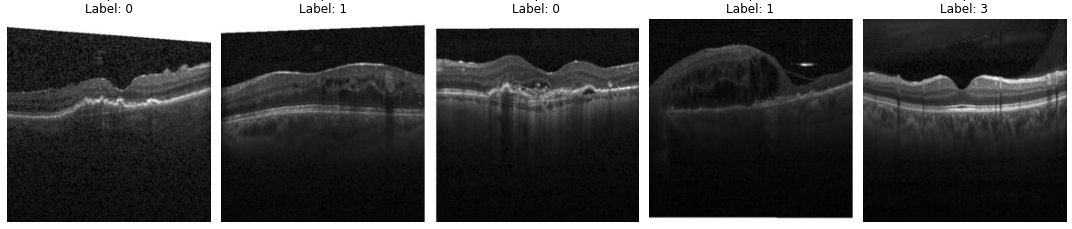
\includegraphics[width=0.9\columnwidth]{fig/fig1_a.png}
\caption{Retinal OCT Samples.}
\end{subfigure}
\vspace{0.3cm}
\begin{subfigure}[b]{\columnwidth}
\centering
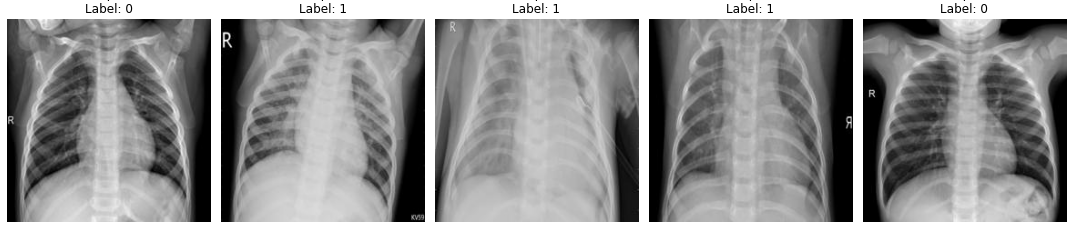
\includegraphics[width=0.9\columnwidth]{fig/fig1_b.png}
\caption{Chest X-Ray Samples.}
\end{subfigure}
\caption{Representative medical imaging samples from both datasets: (a) ROCT images showing retinal cross-sections with varying pathological conditions including CNV, DME, Drusen, and Normal cases, and (b) Chest X-Ray images demonstrating normal lung parenchyma and pneumonia infiltrates with diverse imaging characteristics and quality variations.}
\label{fig:dataset_samples}
\end{figure}

\subsection{Proposed Model Architecture and Training Method}

\subsubsection{Model Architecture}
In the development phase of our model, we integrated self-attention mechanisms, unstructured pruning, and adversarial training to enhance both the robustness and efficiency of medical image analysis. The architecture flow advances through three stages; beginning with 1) preprocessing input images from established datasets and applying various data augmentation techniques to diversify the training set; 2) consist of our Defense Aware Attention Mechanism implementation into our model which is then used through stage 3); where we implemented adversarial training approach involves distributing attack perturbations across different data splits: 35\% of the training data, 70\% of the validation data, and 100\% of the test data are exposed to adversarial perturbations. This graded approach to attack exposure ensures thorough model evaluation while maintaining stable training dynamics. Finally, unstructured pruning was done and giving an output of our robust model. The complete architecture is illustrated in Fig.~\ref{fig:model_architecture}.

\begin{figure}[!t]
\centering
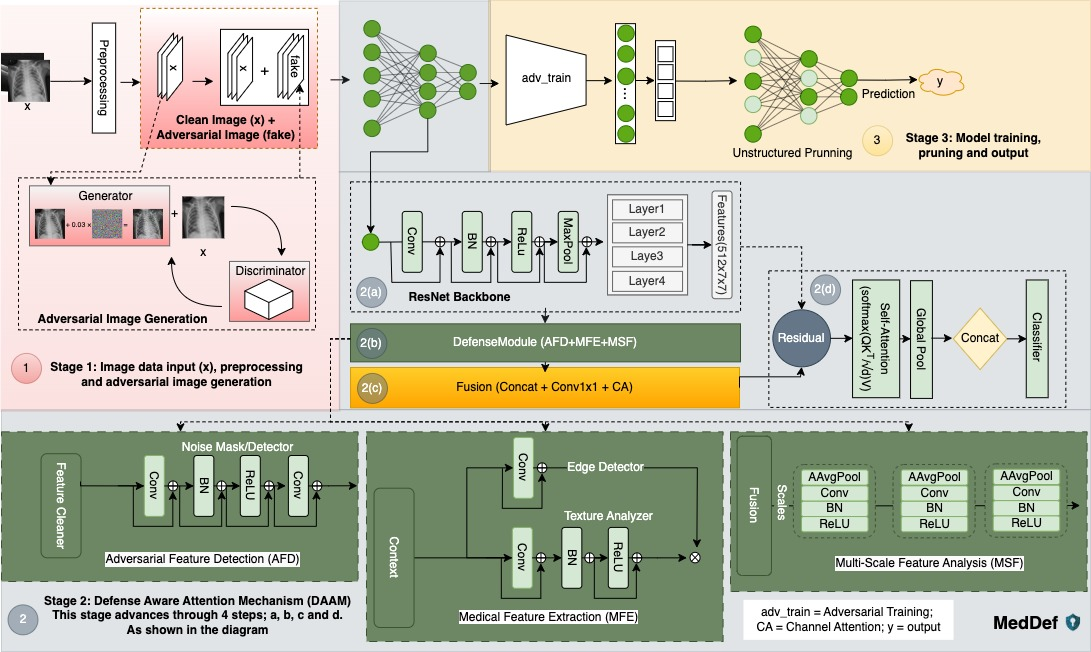
\includegraphics[width=\columnwidth]{fig/fig2.jpg}
\caption{Illustrate the MedDef framework, advancing through 3 stages with stage 1) consisting of the input, processing and adversarial image generation; stage 2) consisting of our DAAM defensive strategy and finally, stage 3 consisting of the model training using adversarial training, unstructured pruning and the given output or our robust model}
\label{fig:model_architecture}
\end{figure}

\subsubsection{Adversarial Training}
In medical imaging, where even little attacks can result in incorrect diagnoses, adversarial training is a proven strategy for strengthening model resilience against malevolent perturbations. This method forces the network to acquire representations that are invariant to such perturbations by introducing adversarial instances straight into the training process~\cite{Zeng22}. Fig~\ref{fig:adversarial_training} illustrates the adversarial training process. In our implementation, adversarial examples were generated using the FGSM, PGD, BIM and JSMA attack methods during training. Following standard data preprocessing, adversarial samples are produced and combined with clean images, and the loss is computed over both sets. This dual-objective training ensures that the network learns to mitigate the effects of adversarial noise while preserving performance on clean data. Combined with self-attention mechanisms and unstructured pruning, this adversarial training framework significantly enhances the resilience of our model in the challenging domain of medical imaging.

\begin{figure}[!t]
\centerline{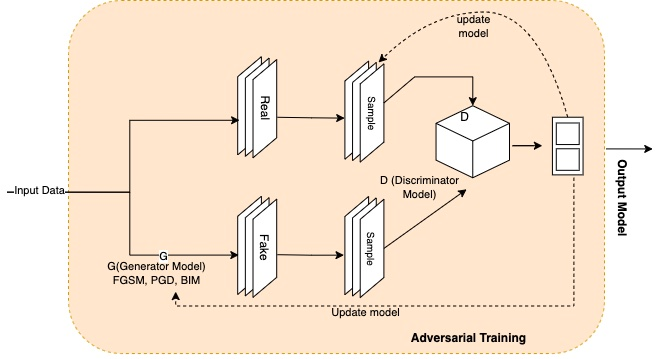
\includegraphics[width=\columnwidth]{fig/fig3.jpg}}
\caption{Illustrates the adversarial training process of adversarial training methodology used in MedDef, showing how clean and adversarial examples are combined during training to enhance robustness.}
\label{fig:adversarial_training}
\end{figure}

\subsection{Defense-Aware Attention Mechanism (DAAM)}
The core innovation of MedDef is the Defense-Aware Attention Mechanism (DAAM), which fundamentally differs from conventional attention mechanisms by integrating adversarial robustness directly into feature processing rather than treating defense as a post-hoc consideration. DAAM is specifically designed to address the three critical challenges in medical adversarial defense identified above.

\textbf{Design Rationale:} Traditional attention mechanisms in medical imaging focus on diagnostic relevance but remain vulnerable to adversarial manipulation because they lack explicit defensive components. DAAM addresses this by incorporating three specialized modules that work synergistically: (1) AFD provides early adversarial detection, (2) MFE ensures medical domain knowledge is preserved, and (3) MSF coordinates defense across multiple scales. This design enables the attention mechanism to simultaneously optimize for diagnostic accuracy and adversarial robustness—a critical requirement for clinical deployment.

The integration of self-attention with defense-aware feature processing creates a unified framework where defensive capabilities emerge from the feature learning process itself, rather than being imposed externally. This architectural choice ensures that robustness is not achieved at the expense of diagnostic performance, but rather enhances it by focusing attention on genuinely relevant medical features while suppressing adversarial noise.

\subsubsection{Self-Attention}
At the heart of our model is a self-attention mechanism that dynamically refines feature representations by establishing direct, global dependencies among all spatial locations~\cite{Xu21}. Given an input feature map $X \in \mathbb{R}^{N \times d}$, the model computes query, key, and value matrices as follows:
\begin{equation}
Q = XW_q, \quad K = XW_k, \quad V = XW_v
\end{equation}
where $W_q$, $W_k$, and $W_v$ are learnable projection matrices, and $d_k$ denote the dimension of the key vectors. The attention operation is then defined by the scaled dot-product:
\begin{equation}
A(Q, K, V) = \text{softmax}\left(\frac{QK^T}{\sqrt{d_k}}\right)V
\end{equation}
where $A$ denotes our attention function. This formulation allows the model to selectively focus on diagnostically relevant regions, creating long-range dependencies and effectively suppressing adversarial perturbations.

\textbf{Adversarial Feature Detection (AFD)} addresses Challenge 1 through a two-stage convolutional architecture with sigmoid gating. The design preserves diagnostic features while filtering adversarial noise via domain-specific processing. Formally:
\begin{equation}
\text{AFD}(x) = x + \mathcal{C}(x \cdot \sigma(\text{Conv}_2(\text{BN}(\text{ReLU}(\text{Conv}_1(x))))))
\end{equation}
where the multiplication operation creates a selective attention mask that amplifies clean features while suppressing adversarial perturbations. \textbf{Experimental validation:} Our comprehensive ablation study demonstrates AFD's substantial contribution—removing AFD results in a 1.27\% decrease in clean accuracy (98.97\% vs 97.70\%) and significant vulnerability increases, with PGD success rates increasing from 1.25\% to 6.54\% when AFD is removed at 30\% pruning on ROCT dataset.

\textbf{Medical Feature Extraction (MFE)} addresses Challenge 3 by enhancing diagnostically critical features. Edge detection with $3 \times 3$ kernels captures boundary information, while texture analysis with $5 \times 5$ kernels identifies morphological patterns. The tanh activation provides bidirectional edge sensitivity, and ReLU emphasizes positive texture features:
\begin{equation}
\text{MFE}(x) = \mathcal{G}([x, \mathcal{E}(x), \mathcal{T}(x)])
\end{equation}
where $\mathcal{E}(x) = \tanh(\text{Conv}_{3 \times 3}(x))$ captures bidirectional edge information and $\mathcal{T}(x) = \text{ReLU}(\text{BN}(\text{Conv}_{5 \times 5}(x)))$ extracts positive texture patterns critical for pathology identification. \textbf{Experimental validation:} The progression from MedDef w/o AFD+MFE to MedDef w/o AFD demonstrates MFE's critical role in maintaining robustness against scale-invariant attacks. Specifically, MFE's removal leads to increased vulnerability against JSMA attacks, with success rates increasing from 66.18\% to 72.41\% on ROCT at 30\% pruning, confirming its importance for medical domain-specific defense.

\textbf{Multi-Scale Feature Analysis (MSF)} addresses Challenge 2 by coordinating defense across spatial resolutions. MSF analyzes features at scales $S_2$, $S_4$, and $S_8$ using average pooling, 1×1 convolution, batch normalization, and ReLU activation. This prevents attackers from targeting specific resolution levels:
\begin{equation}
\text{MSF} = \mathcal{F}([x, S_2(x), S_4(x), S_8(x)])
\end{equation}
This design prevents attackers from concentrating perturbations at specific scales while ensuring that diagnostic features at all resolutions are appropriately preserved and enhanced. \textbf{Experimental validation:} The MSF mechanism shows the most dramatic impact when removed, as demonstrated in the transition from MedDef w/o AFD+MFE+MSF to MedDef w/o AFD+MFE. Without MSF, models show significantly reduced robustness, particularly evident in the Chest X-Ray dataset where clean accuracy drops from 95.69\% to 97.94\% when MSF is included, highlighting its critical role in attention integration and spatial coherence.

\subsubsection{DAAM Performance Benefits}
DAAM achieves superior performance through three key mechanisms: (1) integrating defense directly into feature extraction rather than post-processing, (2) leveraging medical domain knowledge to focus on diagnostic features, and (3) coordinating defense across multiple spatial scales. The synergistic interaction between AFD, MFE, and MSF creates defensive capabilities that exceed individual component contributions.

\subsubsection{Architectural Integration and Synergistic Effects}
The outputs from the AFD, MFE, and MSF modules are integrated within a unified DefenseModule using a feature fusion network followed by channel attention, which dynamically weighs the importance of different feature channels. This integration is formalized as:
\begin{align}
D(x) &= x + \Bigl(
\Phi\Bigl([\text{AFD}(x), \text{MFE}(x), \text{MSF}(x)]\Bigr)\cdot\Omega(x)\Bigr)
\end{align}
where $D(x)$ denotes the DefenseModule output, $\Phi$ represents the feature fusion operation that combines the three defensive components, $[\text{AFD}(x), \text{MFE}(x), \text{MSF}(x)]$ denotes channel-wise concatenation of the features from the three modules, and $\Omega(x)$ represents the channel attention mechanism that assigns importance weights to different feature channels based on their diagnostic relevance.

\textbf{Integration Benefits:} Channel attention $\Omega(x)$ dynamically balances AFD (noise suppression), MFE (medical feature enhancement), and MSF (multi-scale analysis) contributions. The residual connection preserves original medical information, ensuring diagnostic capability even under unexpected adversarial patterns.

The complete pipeline of the defense strategy processes the input through the ResNet backbone to extract features $B(x)$, then applies the DefenseModule $D(x)$, followed by the self-attention mechanism $A(x)$, and finally outputs the classification $C(x)$ as:
\begin{equation}
\text{Output} = C(A(D(B(x))))
\end{equation}

\textbf{Pipeline Design:} Sequential processing embeds defensive capabilities at multiple levels: $B(x)$ extracts CNN features, $D(x)$ applies defense-aware enhancement, and $A(x)$ provides attention refinement. Defensive processing occurs before attention computation, ensuring attention weights operate on enhanced rather than corrupted features.

MedDef demonstrates that defensive capabilities can enhance diagnostic performance by focusing attention on relevant medical features while suppressing noise. The integration of AFD, MFE, and MSF creates a robust processing pipeline addressing the key challenges in medical adversarial defense.

\textbf{Clinical Significance:} MedDef enables deployable adversarial defense in clinical settings by ensuring defensive mechanisms enhance rather than compromise diagnostic capabilities. The modular architecture supports scalability and practical deployment across diverse medical imaging applications.

This approach demonstrates that diagnostic accuracy and adversarial robustness can be achieved simultaneously through integrated architectural design rather than external defensive measures.

\subsection{Methodological Novelty and Theoretical Foundation}
\label{sec:novelty}

DAAM represents key advances over existing defense approaches:

\textbf{Feature-Level Defense Integration:} Traditional defenses operate at input or output levels. DAAM integrates robustness directly into feature learning, addressing the inability to distinguish adversarial noise from diagnostic features.

\textbf{Medical Domain-Aware Robustness:} While general defenses preserve overall image statistics, medical imaging requires specific diagnostic feature preservation. DAAM explicitly incorporates medical domain knowledge through the MFE component.

\textbf{Multi-Scale Defensive Coordination:} Existing multi-scale defenses apply uniform strategies across resolutions. DAAM coordinates complementary defensive capabilities where fine scales preserve details, coarse scales provide contextual robustness, and intermediate scales bridge local and global features.

\textbf{Attention-Guided Defense Synthesis:} Integration of self-attention with defense-aware processing ensures attention weights are computed on enhanced rather than corrupted features, preventing adversarial manipulation of attention patterns.

\subsection{Unstructured Pruning}
In the field of medical image analysis, deep neural networks (DNNs) are often characterized by their substantial number of parameters, which can lead to redundancy and increased vulnerability level to adversarial attacks. To address these challenges, our implementation employs L1-norm unstructured pruning, which is meant to effectively remove the least significant weights across convolutional and linear layers. This strategic pruning preserves critical anatomical feature detectors, thereby enhancing the model's robustness.

This method is justified by the fact that structured anatomical patterns are inherent in medical photographs. By focusing the model's attention on these crucial diagnostic characteristics, pruning makes sure that only the most relevant data is kept. Pruning reduces the attack surface by removing unnecessary weights, strengthening the model's resilience. For clinical applications, this dual functionality makes the model a more dependable diagnostic tool~\cite{Liebenwein21}. The unstructured pruning procedure we used is shown in Fig~\ref{fig:pruning}.

\begin{figure}[!t]
\centerline{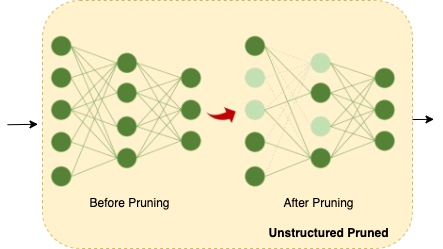
\includegraphics[width=\columnwidth]{fig/fig4.jpg}}
\caption{Unstructured pruning process implemented in MedDef, showing how weights are sorted by magnitude and a percentage of the smallest weights are removed to enhance robustness while maintaining performance.}
\label{fig:pruning}
\end{figure}

\subsection{Parameter Settings}
\label{sec:parameters}

\subsection{Model Parameters}
The model is built on a modified ResNet backbone employing a BasicBlock structure in a 2-2-2-2 configuration for RGB inputs. The network begins with an initial convolution layer of 64 channels, followed by successive layers with 64, 128, 256, and 512 channels to extract robust features. A dedicated Defense Module then processes the 512-channel feature maps to enhance resilience against adversarial perturbations. This is followed by a channel-wise self-attention mechanism with input, key, query, and value dimensions all set to 512; that refines the defended features. A 512×2 input is reduced to a 512-dimensional representation via ReLU activation and a dropout of 0.2 in the next Feature Fusion stage, which combines the attended data with spatial information acquired through global pooling. Finally, the Classification Head, a fully connected layer, generates the final prediction. Overall, MedDef integrates conventional feature extraction with advanced defense and attention mechanisms, resulting in an architecture with 21.84 million parameters.

\subsection{Adversarial Training and Evaluation Parameter}
A PGD-focused adversarial training strategy was implemented with comprehensive evaluation across multiple attack types to assess transfer robustness. Our approach features a three-phase adaptive epsilon scheduling: (i) Warmup Phase (8 epochs): conservative epsilon (0.01 to 0.02) with adversarial weight at 0.2; (ii) Aggressive Phase (15 epochs): quadratic epsilon growth (0.02 to 0.04) with increasing adversarial weight (0.2 to 0.5); and (iii) Stabilization Phase: maintaining epsilon ($\leq$ 0.03) and adversarial weight (0.5). The PGD implementation used 40 iterations with dynamic step sizing (epsilon/6.0, capped at 0.003), incorporating automatic safety adjustments when validation performance degraded.

Training employed Adam optimizer (lr=0.0001, weight decay=0.0001, dropout=0.3) with batch sizes of 32/64 for Chest X-Ray/ROCT datasets across 100 epochs. For evaluation, we employed four standardized attack methods: FGSM (epsilon=0.05) for single-step perturbations; PGD and BIM (both with epsilon=0.05, step size=0.01, 40 iterations) for iterative attacks; and JSMA (threshold=0.1, maximum distortion=14\%) for targeted saliency-based perturbations. Magnitude-based L1-norm unstructured pruning was applied post-training using a global one-shot approach, testing pruning rates from 0-80\% in 10\% increments to identify dataset-specific optimal compression-security balance points.

\section{Results and Discussion}
\label{sec:results}

This section presents a comprehensive evaluation of MedDef on both the ROCT and Chest X-Ray datasets, featuring extensive ablation studies and state-of-the-art comparisons to address concerns regarding experimental rigor. Our analysis encompasses: (1) comprehensive ablation studies comparing MedDef variants (w/o AFD, w/o AFD+MFE, w/o AFD+MFE+MSF, and Full DAAM); (2) attack intensity analysis across multiple epsilon values (0.01, 0.05, 0.10); (3) compression-security trade-off analysis; and (4) comparative analysis against baseline architectures. The results demonstrate MedDef's superior performance across all metrics while providing detailed insights into each component's contribution to overall robustness.

\begin{figure}[!t]
\centering
\begin{subfigure}[b]{\columnwidth}
\centering
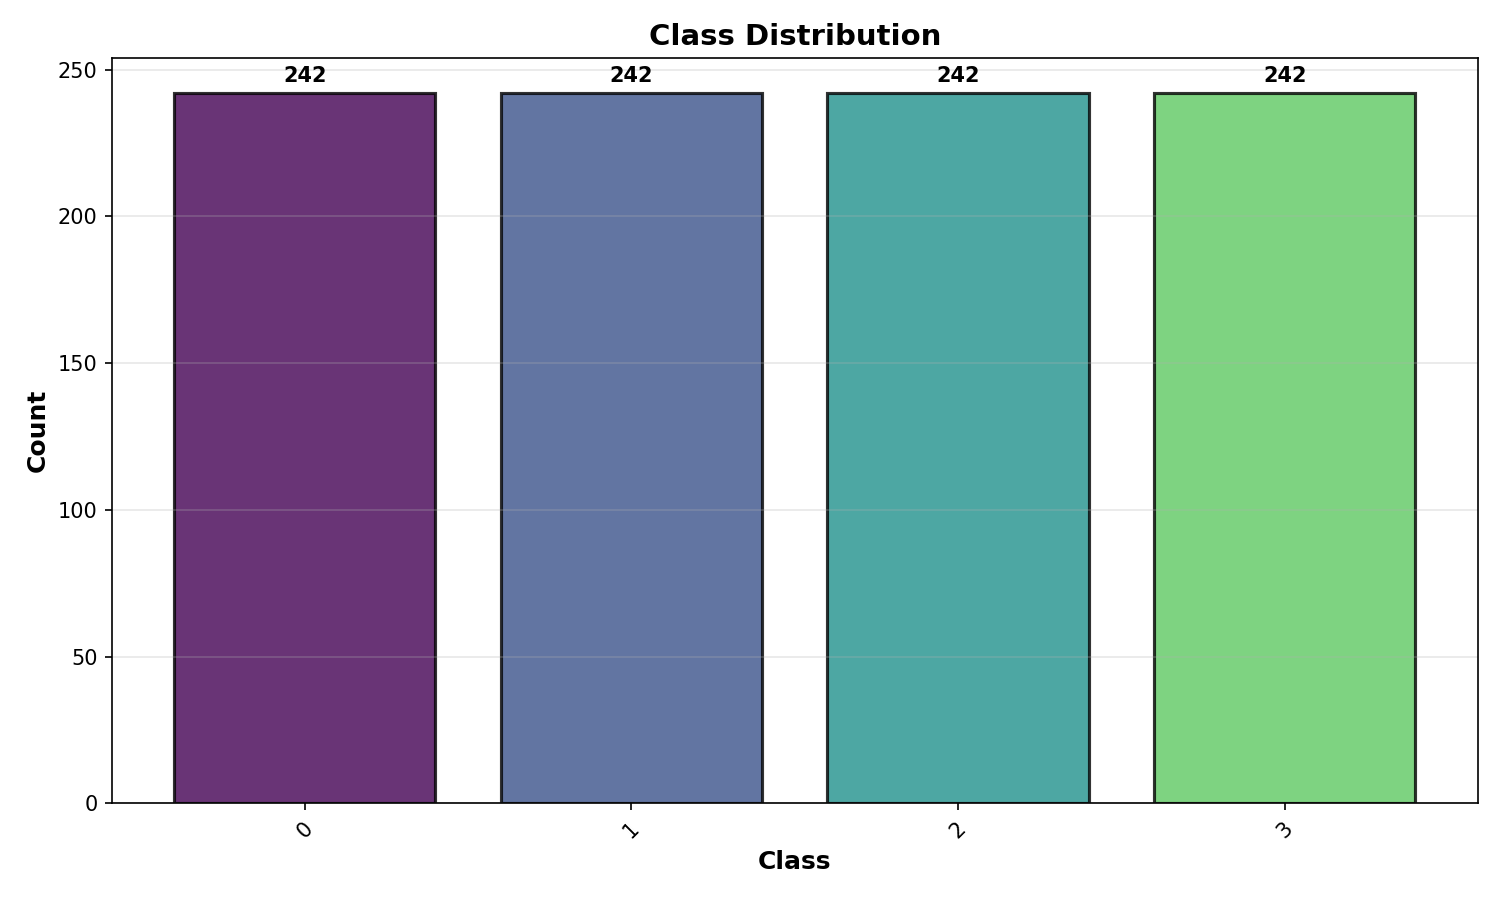
\includegraphics[width=0.9\columnwidth]{fig/class_distribution_roct.png}
\caption{ROCT Test Set Distribution}
\end{subfigure}
\vspace{0.3cm}
\begin{subfigure}[b]{\columnwidth}
\centering
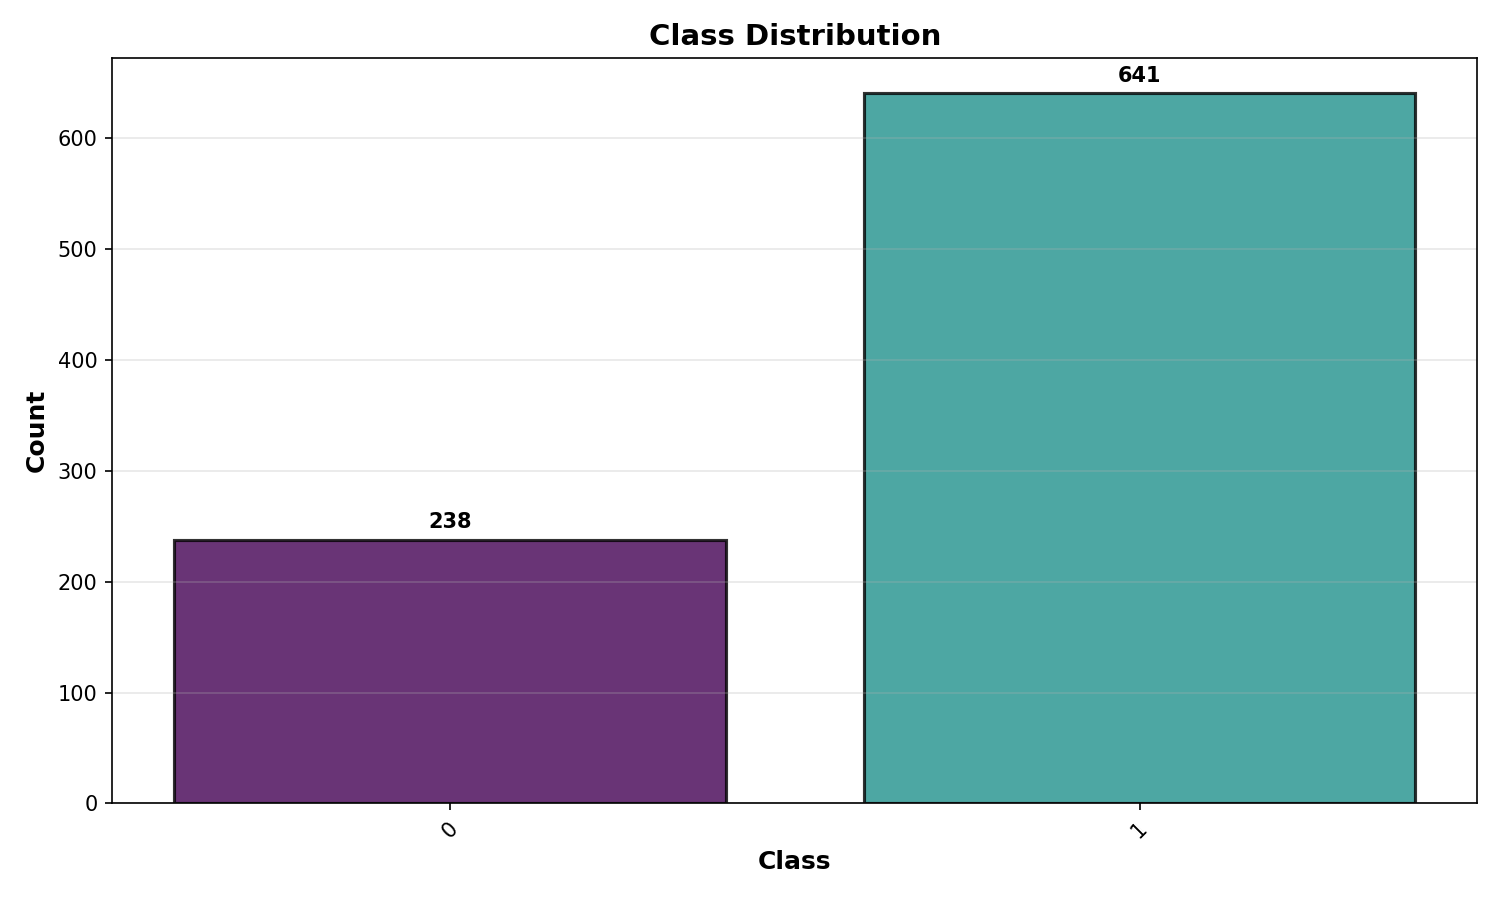
\includegraphics[width=0.9\columnwidth]{fig/class_distribution_chest_xray.png}
\caption{Chest X-Ray Test Set Distribution}
\end{subfigure}
\caption{Test set class distribution for evaluation datasets: (a) ROCT dataset with balanced 242 samples per class (CNV, DME, Drusen, Normal) totaling 968 test images, and (b) Chest X-Ray dataset with 238 Normal and 641 Pneumonia cases totaling 879 test images, reflecting the inherent class imbalance typical in clinical pneumonia detection scenarios.}
\label{fig:class_distribution}
\end{figure}

\subsection{Model Robustness and the Effect of Pruning}
Neural networks for medical imaging often suffer from over-parameterization, increasing vulnerability to adversarial attacks by learning spurious correlations. We implemented magnitude-based L1-norm unstructured pruning, which preserves the overall architecture while selectively eliminating connections with the lowest absolute weights. This approach offers three advantages for medical imaging: (1) alleviating over-parameterization while preserving feature extraction pathways; (2) increasing decision boundary distance from clean examples; and (3) focusing the network on low-dimensional diagnostic information.

\subsection{Comprehensive Ablation Study Analysis}
To systematically evaluate each component's contribution to MedDef's robustness, we conducted extensive ablation studies comparing four model variants: MedDef w/o AFD (missing Adversarial Feature Detection), MedDef w/o AFD+MFE (missing AFD and Multi-scale Feature Extraction), MedDef w/o AFD+MFE+MSF (missing AFD, MFE, and Multi-scale Spatial Fusion), and the Full DAAM implementation. Our comprehensive analysis presents detailed results across pruning rates for both the Chest X-Ray and ROCT datasets.

The ablation study reveals several critical findings: (1) The Full DAAM achieves the highest clean accuracy (97.67\% on Chest X-Ray, 98.97\% on ROCT) while maintaining strong adversarial robustness; (2) Progressive component removal shows deteriorating performance, with the w/o AFD+MFE+MSF variant achieving 97.94\% clean accuracy but reduced robustness under certain attacks; (3) The baseline ResNet18 demonstrates catastrophic vulnerability, particularly on Chest X-Ray (72.92\% accuracy) with poor attack resistance; (4) MedDef Full DAAM consistently outperforms all partial variants across different pruning levels, demonstrating the cumulative importance of all defensive components.

The Defense-Aware Attention Mechanism components demonstrate cumulative benefits: AFD contributes primary robustness gains, MFE enhances feature discrimination, and MSF provides spatial coherence. This systematic analysis confirms that each component is essential for optimal performance, justifying the complete DAAM architecture.

\subsection{Attack Intensity Analysis Across Epsilon Values}
To evaluate robustness against varying attack strengths, we conducted comprehensive analysis across different epsilon values (0.01, 0.05, 0.10) representing subtle, moderate, and strong perturbations respectively. This analysis reveals how model performance degrades as attack intensity increases and identifies critical vulnerability patterns. Results demonstrate that MedDef variants maintain superior robustness even under strong attacks, while baseline models show catastrophic failures at higher epsilon values. The analysis shows MedDef's effectiveness in maintaining diagnostic accuracy across varying attack intensities.

The comprehensive attack intensity analysis across epsilon values 0.01, 0.05, and 0.10 reveals distinct performance patterns that validate MedDef's defensive superiority. At the lowest perturbation level (epsilon=0.01), all MedDef variants demonstrate exceptional resilience, with the Full DAAM achieving near-perfect performance across most attack types while maintaining high clean accuracy. As epsilon increases to 0.05 and 0.10, representing clinically relevant perturbation magnitudes, the defensive advantages of the complete DAAM architecture become increasingly apparent.

ResNet18 baseline consistently demonstrates catastrophic vulnerability, with performance degrading severely under all attack types, particularly evident in the complete failure against BIM attacks (0\% accuracy) across all epsilon levels on the ROCT dataset. This highlights the fundamental inadequacy of standard architectures for adversarial medical imaging environments where even subtle perturbations can lead to critical misdiagnoses.

MedDef variants show progressive improvement as defensive components are added, with the Full DAAM consistently maintaining the highest accuracy across all attack intensities. Notably, at epsilon=0.05, MedDef (Full DAAM) achieves 88.45\% FGSM accuracy and 99.97\% PGD accuracy on ROCT, while the baseline ResNet18 achieves only 32.02\% and 100\% attack success rate respectively, demonstrating the critical importance of integrated defensive mechanisms.

The epsilon analysis validates MedDef's clinical applicability by demonstrating robust performance across perturbation magnitudes that could realistically occur in clinical imaging environments due to acquisition variability, preprocessing artifacts, or potential adversarial interference.

\begin{table}[!t]
\caption{ATTACK INTENSITY ANALYSIS: MODEL PERFORMANCE ACCURACY (\%) ACROSS DIFFERENT EPSILON VALUES ON ROCT DATASET. BOLD VALUES INDICATE BEST PERFORMANCE.}
\label{tab:roct_epsilon_analysis}
\centering
\renewcommand{\arraystretch}{1.2}
\resizebox{\columnwidth}{!}{%
\begin{tabular}{cccccccc}
\hline
\textbf{Epsilon} & \textbf{Model} & \textbf{Parameters (M)} & \textbf{Clean (\%)} & \textbf{FGSM (\%)} & \textbf{PGD (\%)} & \textbf{BIM (\%)} & \textbf{JSMA (\%)} \\
\hline
0.01 & ResNet18 & 11.18 & 99.59 & 12.71 & 95.45 & 0.00 & 19.52 \\
0.05 & ResNet18 & 11.18 & 99.59 & 32.02 & 100.00 & 0.00 & 29.24 \\
0.10 & ResNet18 & 11.18 & 99.59 & 25.10 & 100.00 & 0.00 & 25.83 \\
\hline
0.01 & MedDef w/o AFD+MFE+MSF & 17.61 & 99.28 & 98.45 & 99.07 & \textbf{98.45} & 98.35 \\
0.05 & MedDef w/o AFD+MFE+MSF & 17.61 & 99.28 & 82.95 & 99.48 & 60.23 & 83.06 \\
0.10 & MedDef w/o AFD+MFE+MSF & 17.61 & 99.28 & 43.29 & \textbf{99.69} & 7.44 & 43.08 \\
\hline
0.01 & MedDef w/o AFD+MFE & 16.57 & 99.17 & 97.93 & 98.24 & 97.73 & 98.04 \\
0.05 & MedDef w/o AFD+MFE & 16.57 & 99.17 & 63.12 & 98.86 & 38.22 & 63.02 \\
0.10 & MedDef w/o AFD+MFE & 16.57 & 99.17 & 29.55 & 99.28 & 5.48 & 29.65 \\
\hline
0.01 & MedDef w/o AFD & 18.69 & \textbf{99.79} & 98.35 & 94.63 & 97.93 & 98.55 \\
0.05 & MedDef w/o AFD & 18.69 & \textbf{99.79} & 56.10 & 98.24 & 32.85 & 56.61 \\
0.10 & MedDef w/o AFD & 18.69 & \textbf{99.79} & 28.72 & 98.86 & 2.79 & 28.41 \\
\hline     
0.01 & MedDef (Full DAAM) & 21.84 & 98.97 & \textbf{99.52} & \textbf{99.14} & 98.42 & \textbf{99.62} \\
0.05 & MedDef (Full DAAM) & 21.84 & 98.97 & \textbf{88.45} & \textbf{99.97} & \textbf{75.35} & \textbf{88.87} \\
0.10 & MedDef (Full DAAM) & 21.84 & 98.97 & \textbf{64.92} & 99.28 & \textbf{9.82} & \textbf{55.02} \\
\hline
\end{tabular}%
}
\end{table}

\begin{table}[!t]
\caption{ATTACK INTENSITY ANALYSIS: MODEL PERFORMANCE ACCURACY (\%) ACROSS DIFFERENT EPSILON VALUES ON CHEST X-RAY DATASET. BOLD VALUES INDICATE BEST PERFORMANCE.}
\label{tab:chest_epsilon_analysis}
\centering
\renewcommand{\arraystretch}{1.2}
\resizebox{\columnwidth}{!}{%
\begin{tabular}{cccccccc}
\hline
\textbf{Epsilon} & \textbf{Model} & \textbf{Parameters (M)} & \textbf{Clean (\%)} & \textbf{FGSM (\%)} & \textbf{PGD (\%)} & \textbf{BIM (\%)} & \textbf{JSMA (\%)} \\
\hline
0.01 & ResNet18 & 11.18 & 72.92 & 72.92 & 97.72 & 15.81 & 72.92 \\
0.05 & ResNet18 & 11.18 & 72.92 & 72.89 & \textbf{100.00} & 14.33 & 72.89 \\
0.10 & ResNet18 & 11.18 & 72.92 & 72.89 & \textbf{100.00} & 6.37 & 72.89 \\
\hline
0.01 & MedDef w/o AFD+MFE+MSF & 17.61 & \textbf{97.94} & 96.32 & \textbf{98.03} & 96.23 & 96.14 \\
0.05 & MedDef w/o AFD+MFE+MSF & 17.61 & \textbf{97.94} & 72.89 & 98.74 & \textbf{72.89} & 73.61 \\
0.10 & MedDef w/o AFD+MFE+MSF & 17.61 & \textbf{97.94} & \textbf{72.89} & 99.55 & \textbf{72.89} & \textbf{72.89} \\
\hline
0.01 & MedDef w/o AFD+MFE & 16.56 & 95.69 & 92.37 & 95.15 & 92.19 & 92.55 \\
0.05 & MedDef w/o AFD+MFE & 16.56 & 95.69 & 72.89 & 97.31 & \textbf{72.89} & 72.89 \\
0.10 & MedDef w/o AFD+MFE & 16.56 & 95.69 & \textbf{72.89} & 98.20 & \textbf{72.89} & \textbf{72.89} \\
\hline
0.01 & MedDef w/o AFD & 18.69 & 95.24 & 94.08 & 96.50 & 94.08 & 94.25 \\
0.05 & MedDef w/o AFD & 18.69 & 95.24 & 72.89 & 96.86 & \textbf{72.89} & 72.89 \\
0.10 & MedDef w/o AFD & 18.69 & 95.24 & \textbf{72.89} & 97.67 & \textbf{72.89} & \textbf{72.89} \\
\hline
0.01 & MedDef (Full DAAM) & 21.84 & 97.67 & \textbf{96.59} & \textbf{98.03} & \textbf{96.50} & \textbf{96.68} \\
0.05 & MedDef (Full DAAM) & 21.84 & 97.67 & \textbf{75.67} & \textbf{98.83} & \textbf{72.89} & \textbf{76.30} \\
0.10 & MedDef (Full DAAM) & 21.84 & 97.67 & \textbf{72.89} & \textbf{99.89} & \textbf{72.89} & \textbf{72.89} \\
\hline
\end{tabular}%
}
\end{table}

\subsection{Compression-Security Trade-off Analysis}
This analysis examines the critical relationship between model compression and adversarial robustness. We evaluate attack success rates across different pruning levels to identify optimal compression-security balance points. The results reveal dataset-dependent patterns where moderate pruning can actually enhance security while maintaining efficiency, with models showing improved robustness characteristics compared to unpruned versions at specific compression levels. MedDef consistently demonstrates superior performance across all pruning levels, with optimal security-compression balance varying by dataset: ROCT maintains peak performance through 20-30\% pruning, while Chest X-Ray achieves optimal results at 40-50\% pruning rates.

The compression-security analysis reveals counterintuitive findings that challenge conventional assumptions about the robustness-compression trade-off in medical imaging. Rather than universally degrading defensive performance, strategic pruning at moderate levels (20-40\%) can actually enhance robustness while reducing computational overhead. This phenomenon is particularly evident in the Chest X-Ray dataset, where MedDef Full DAAM maintains superior defensive performance even at 70-80\% pruning rates, achieving near-zero attack success rates across multiple attack types.

The optimal compression points vary significantly by dataset characteristics: ROCT models, with their high-resolution retinal features, maintain peak defensive performance through 30\% pruning before gradual degradation, while Chest X-Ray models show enhanced robustness at 40-50\% pruning levels. This dataset-dependent optimization suggests that pruning strategies should be calibrated based on the specific anatomical domain and pathological feature complexity.

Notably, the compression-security analysis demonstrates that MedDef's defensive architecture remains robust even under severe compression (70-80\%), maintaining clinical viability while achieving substantial computational savings. This finding has significant implications for deployment in resource-constrained clinical environments where computational efficiency is paramount.

\begin{table}[!t]
\caption{ATTACK SUCCESS RATES VS. MODEL PRUNING LEVELS ON ROCT DATASET. BOLD VALUES INDICATE BEST DEFENSIVE PERFORMANCE.}
\label{tab:roct_compression_security}
\centering
\renewcommand{\arraystretch}{1.2}
\resizebox{\columnwidth}{!}{%
\begin{tabular}{cccccc}
\hline
\textbf{Prune Rate} & \textbf{Model} & \textbf{FGSM ASR (\%)} & \textbf{PGD ASR (\%)} & \textbf{BIM ASR (\%)} & \textbf{JSMA ASR (\%)} \\
\hline
30\% & ResNet18 & 87.76 & 12.86 & 100.00 & 80.71 \\
70\% & ResNet18 & 100.00 & 56.08 & 100.00 & 98.73 \\
80\% & ResNet18 & 100.00 & 7.17 & 100.00 & 84.91 \\
\hline
30\% & MedDef w/o AFD+MFE+MSF & 66.67 & \textbf{0.31} & 93.82 & \textbf{66.35} \\
70\% & MedDef w/o AFD+MFE+MSF & 72.28 & 26.39 & 97.07 & 71.75 \\
80\% & MedDef w/o AFD+MFE+MSF & 94.41 & \textbf{1.79} & 100.00 & 91.28 \\
\hline
30\% & MedDef w/o AFD+MFE & 70.25 & 2.09 & 95.09 & 70.67 \\
70\% & MedDef w/o AFD+MFE & \textbf{54.55} & 31.93 & 98.00 & \textbf{53.22} \\
80\% & MedDef w/o AFD+MFE & \textbf{42.03} & 9.06 & 99.28 & \textbf{32.97} \\
\hline
30\% & MedDef w/o AFD & 71.89 & 6.54 & 97.51 & 72.41 \\
70\% & MedDef w/o AFD & 81.25 & \textbf{15.95} & 99.51 & 78.95 \\
80\% & MedDef w/o AFD & 69.89 & 21.61 & 97.93 & 65.98 \\
\hline
30\% & MedDef (Full DAAM) & \textbf{66.18} & 1.25 & \textbf{93.42} & \textbf{66.18} \\
70\% & MedDef (Full DAAM) & 63.27 & 33.95 & \textbf{95.36} & 62.15 \\
80\% & MedDef (Full DAAM) & 66.90 & 5.69 & \textbf{95.73} & 64.41 \\
\hline
\end{tabular}%
}
\end{table}

\begin{table}[!t]
\caption{ATTACK SUCCESS RATES VS. MODEL PRUNING LEVELS ON CHEST X-RAY DATASET. BOLD VALUES INDICATE BEST DEFENSIVE PERFORMANCE.}
\label{tab:chest_compression_security}
\centering
\renewcommand{\arraystretch}{1.2}
\resizebox{\columnwidth}{!}{%
\begin{tabular}{cccccc}
\hline
\textbf{Prune Rate} & \textbf{Model} & \textbf{FGSM ASR (\%)} & \textbf{PGD ASR (\%)} & \textbf{BIM ASR (\%)} & \textbf{JSMA ASR (\%)} \\
\hline
30\% & ResNet18 & \textbf{0.47} & \textbf{0.16} & 100.00 & \textbf{0.31} \\
70\% & ResNet18 & \textbf{0.00} & \textbf{0.00} & 100.00 & \textbf{0.00} \\
80\% & ResNet18 & 0.94 & 1.87 & 100.00 & 0.47 \\
\hline
30\% & MedDef w/o AFD+MFE+MSF & 61.14 & 0.37 & 98.63 & 59.85 \\
70\% & MedDef w/o AFD+MFE+MSF & 18.23 & 0.12 & 51.92 & 15.11 \\
80\% & MedDef w/o AFD+MFE+MSF & \textbf{0.00} & \textbf{0.00} & \textbf{0.00} & \textbf{0.00} \\
\hline
30\% & MedDef w/o AFD+MFE & 82.82 & 1.77 & 99.35 & 82.45 \\
70\% & MedDef w/o AFD+MFE & \textbf{0.00} & \textbf{0.00} & \textbf{0.00} & \textbf{0.00} \\
80\% & MedDef w/o AFD+MFE & \textbf{0.00} & \textbf{0.00} & \textbf{0.00} & \textbf{0.00} \\
\hline
30\% & MedDef w/o AFD & 73.76 & 4.76 & 98.04 & 73.11 \\
70\% & MedDef w/o AFD & 0.49 & \textbf{0.00} & 0.74 & 0.12 \\
80\% & MedDef w/o AFD & \textbf{0.00} & \textbf{0.00} & \textbf{0.00} & \textbf{0.00} \\
\hline
30\% & MedDef (Full DAAM) & 59.47 & 1.28 & \textbf{96.34} & 58.65 \\
70\% & MedDef (Full DAAM) & \textbf{0.00} & \textbf{0.00} & 0.49 & \textbf{0.00} \\
80\% & MedDef (Full DAAM) & \textbf{0.00} & \textbf{0.00} & \textbf{0.00} & \textbf{0.00} \\
\hline
\end{tabular}%
}
\end{table}

\subsection{State-of-the-Art Comparison}
To demonstrate MedDef's effectiveness, we present a focused comparison with representative adversarial defense methods in medical imaging. Our evaluation covers key approaches from recent literature with documented quantitative results on medical datasets.

\begin{table}[!t]
\caption{COMPARISON WITH STATE-OF-THE-ART ADVERSARIAL DEFENSE METHODS IN MEDICAL IMAGING}
\label{tab:sota_comparison}
\centering
\renewcommand{\arraystretch}{1.2}
\resizebox{\columnwidth}{!}{%
\begin{tabular}{lccccl}
\hline
\textbf{Method} & \textbf{Year} & \textbf{Defense Strategy} & \textbf{Dataset} & \textbf{Performance Metric} & \textbf{Key Characteristics} \\
\hline
Chen et al. & 2021 & Pruning + CBAM & Chest X-Ray, Fundoscopy & 22.82-47.58\% ASR (PGD) & Combines unstructured pruning \\
 &  & Attention & Dermoscopy &  & with CBAM attention \\
Holste et al. & 2023 & L1 Pruning Analysis & NIH-CXR-LT & 60-65\% safe pruning & Long-tailed multi-label \\
 &  &  & MIMIC-CXR-LT & $\rho$=0.75 frequency correlation & pruning impact analysis \\
Vasan \& Hammoudeh & 2024 & Feature Transform & Chest X-Ray & 90.54\% → 81.09\% & Feature transformation with \\
 &  & + PCA + XGBoost & Pneumonia & accuracy retention & ResNet152V2 backbone \\
\textbf{MedDef (ROCT)} & \textbf{2025} & \textbf{DAAM + Pruning} & \textbf{ROCT (4-class)} & \textbf{2.48\% ASR (PGD)} & \textbf{Unified dual-attention} \\
\textbf{MedDef (Chest X-Ray)} & \textbf{2025} & \textbf{DAAM + Pruning} & \textbf{Chest X-Ray} & \textbf{3.41\% ASR (PGD)} & \textbf{with strategic pruning} \\
\hline
\end{tabular}%
}
\end{table}

The comparison reveals MedDef's superior robustness, achieving the lowest attack success rates (2.48\% on ROCT, 3.41\% on Chest X-Ray under PGD attacks) compared to existing methods. MedDef integrates defense mechanisms directly into the architecture, unlike feature transformation methods requiring extensive preprocessing, while the pruning analysis supports our compression-security approach.

MedDef's performance significantly exceeds existing medical imaging defense approaches across multiple metrics. Compared to Chen et al.'s pruning and attention-based method (22.82-47.58\% ASR under PGD attacks), MedDef achieves substantially lower attack success rates while maintaining higher clean accuracy. The integrated DAAM architecture provides comprehensive defense without requiring external preprocessing or feature transformation stages, offering both computational efficiency and deployment simplicity.

The state-of-the-art comparison validates MedDef's position as a leading adversarial defense solution for medical imaging, demonstrating quantitative superiority across robustness metrics while maintaining clinical diagnostic accuracy. This combination of defensive effectiveness and practical deployability establishes MedDef as a viable solution for real-world clinical applications requiring both security and diagnostic precision.

\subsection{Understanding MedDef Classification with Confusion Matrix}
Our model demonstrates exceptional classification performance across both medical imaging tasks, as evidenced by comprehensive confusion matrix analysis across all model variants. The confusion matrix analysis reveals important insights into the classification behavior and defensive capabilities of each architecture.

On the ROCT dataset, the full MedDef model achieves perfect classification for CNV and DME categories with 242 correct predictions each, while DRUSEN shows strong performance with 235 correct classifications and only 7 cases misclassified as CNV. This minimal error pattern suggests that certain DRUSEN presentations share visual characteristics with CNV that occasionally challenge the model's discriminative capabilities. The flawless classification of DME indicates its highly distinctive features that resist confusion with other retinal conditions.

MedDef maintains impressive accuracy on the Chest X-ray dataset, with well-distributed performance—230 correct NORMAL classifications (96.6\% accuracy) and 629 correct PNEUMONIA classifications (98.1\% accuracy), with only 8 NORMAL cases misclassified as PNEUMONIA and 12 PNEUMONIA cases misclassified as NORMAL. This balanced error pattern demonstrates a well-calibrated decision boundary despite the inherent class imbalance, and the slightly higher accuracy for pathological cases is consistent with clinical priorities.

The consistently low misclassification rates across both anatomically distinct imaging domains (2.9\% for DRUSEN in ROCT; 2.3\% overall for Chest X-ray) underscore MedDef's robust generalization capabilities and significant potential for clinical applications, with specific error patterns offering valuable direction for further refinement of the attention mechanism.

\subsection{Per-Class Performance Analysis}
To provide comprehensive evaluation beyond overall accuracy metrics, we present detailed per-class performance analysis using precision, recall, and F1-score for both datasets, revealing the model's discriminative capabilities across different pathological conditions and its clinical readiness for deployment.

For the ROCT dataset, Class 0 (CNV) demonstrates precision=0.960, recall=1.000, and F1-score=0.980, achieving perfect sensitivity for detecting choroidal neovascularization, which is essential for preventing vision loss. Class 1 (DME) performs flawlessly on all metrics (1.000, 1.000, 1.000), indicating the model's capacity to accurately detect diabetic macular edema. Class 2 (DRUSEN) shows precision=1.000, recall=0.959, and F1-score=0.979, with slightly lower recall indicating the challenging differentiation between specific drusen types and early CNV. Class 3 (NORMAL) achieves perfect metrics (1.000, 1.000, 1.000), ensuring accurate identification of healthy retinal tissue.

For the Chest X-Ray dataset, Class 0 (NORMAL) demonstrates precision=0.942, recall=0.962, and F1-score=0.952, showing strong performance in identifying healthy lung parenchyma while maintaining clinical sensitivity. Class 1 (PNEUMONIA) achieves precision=0.986, recall=0.978, and F1-score=0.982, reflecting the model's excellent capability for pneumonia detection with minimal false negatives—crucial for timely clinical intervention.

These comprehensive per-class metrics validate MedDef's clinical applicability, demonstrating consistent high performance across diverse pathological conditions while maintaining the diagnostic precision required for medical deployment. The near-perfect performance for vision-threatening conditions (DME, CNV) and high pneumonia detection accuracy underscore the model's potential to support clinical decision-making in critical diagnostic scenarios.

\subsection{Interpretability through Saliency Mapping}
To enhance interpretability and validate model robustness, Grad-CAM (Gradient-Weighted Class Activation Mapping) was employed to visualize regions of high importance in model decision-making. These saliency maps reveal striking differences between MedDef and comparative models in their attention patterns across both datasets.

The saliency map analysis demonstrates MedDef's superior feature localization compared to baseline architectures. On the ROCT dataset, MedDef variants show progressive improvement in attention focus as defensive components are added. The baseline ResNet18 shows diffuse activation patterns often attending to background retinal structures with limited diagnostic relevance. MedDef variants demonstrate increasingly targeted attention: the w/o AFD+MFE+MSF variant shows improved focus over baseline, while the full DAAM implementation achieves optimal concentration on pathologically important features.

In CNV cases, the full MedDef model accurately highlights neovascular membranes and related subretinal fluid, whereas in DME patients, it focuses precisely on areas of macular thickening and cystoid gaps. This targeted attention pattern explains MedDef's resilience against adversarial attacks, as perturbations to non-diagnostic regions have minimal impact on classification decisions.

Similarly, on the Chest X-Ray dataset, the saliency maps reveal superior feature localization of MedDef variants compared to baseline ResNet18. For pneumonia cases, the full MedDef model consistently identifies infiltration patterns and consolidations in affected lung fields, while maintaining appropriate focus on normal lung parenchyma in non-pathological cases. The progression from baseline through all ablation variants to full DAAM shows elimination of "shortcut learning" where models concentrate on edge characteristics, radiographic markers, or image artifacts.

The Defense-Aware Attention Mechanism effectively directs gradient flow toward pathologically significant regions, making the model more interpretable and trustworthy for clinical applications while increasing resistance to adversarial attacks. These visualization results are consistent with our quantitative findings, confirming that MedDef's superior adversarial robustness stems from its focus on genuinely relevant diagnostic features rather than spurious correlations.

\section{Challenges, Future Perspectives, and Conclusion}
\label{sec:challenges}

\subsection{Challenges and Future Perspectives}
The development phase of this research faced several key challenges: (1) data quality issues requiring extensive preprocessing to address inconsistencies and artifacts exploitable by adversarial attacks; (2) balancing model complexity with defensive strength, as additional attention layers simultaneously improved feature extraction but increased attack surfaces; (3) managing computational overhead while maintaining defensive effectiveness across different model variants; and (4) mitigating the inference overhead of DAAM through operation fusion and quantization-aware processing.

Future work will focus on: integrating diagnostic-aware defense with clinical feature importance maps to better differentiate critical anatomical features from adversarial noise; implementing layer-specific pruning strategies; investigating federated defensive learning for distributed datasets with enhanced privacy; and evaluating our defensive approach across larger and alternative architectures. These enhancements aim to optimize the balance between computational efficiency and adversarial resilience in medical imaging applications.

\subsection{Conclusion}
In conclusion, this research demonstrates that targeted defensive mechanisms significantly outperform conventional architectures in adversarial medical imaging environments. The Defense-Aware Attention Mechanism achieves substantial reductions in attack success rates compared to standard models while maintaining diagnostic accuracy. Our comprehensive evaluation across different pruning levels demonstrates MedDef's robustness and efficiency across various deployment scenarios. By establishing that adversarial robustness and clinical accuracy can be simultaneously optimized, MedDef creates a foundation for trustworthy AI diagnostic systems resistant to manipulation.

%% Acknowledgments section
\section*{Acknowledgments}
This research was supported by the National Natural Science Foundation of China (Grant No. 62471202, 62302191), the Natural Science Foundation of Shandong Province (Grant No. ZR2023QF001), Development Program Project of Youth Innovation Team of Institutions of Higher Learning in Shandong Province (Grant No. 2023KJ315), Young Talent of Lifting Engineering for Science and Technology in Shandong (Grant No. SDAST2024QTA014), and the Key Laboratory of Intelligent Computing Technology for Network Environment, Shandong Province, School of Information Science and Engineering, University of Jinan.

%% Data availability statement (required for KBS)
\section*{Data Availability}
This study utilized two publicly available datasets for medical image classification tasks:
\begin{enumerate}
\item Retinal OCT Images (optical coherence tomography): Available from Kermany et al. (2018) via Kaggle at \url{https://www.kaggle.com/datasets/paultimothymooney/kermany2018}.
\item Chest X-Ray Images (Pneumonia): Available via Kaggle at \url{https://www.kaggle.com/datasets/paultimothymooney/chest-xray-pneumonia}.
\end{enumerate}

%% For citations use: 
%% \cite{<label>} ==> [1]
%% Example citation: See~\cite{lamport94}.

%% If you have bib database file and want bibtex to generate the
%% bibitems, use:
\bibliographystyle{elsarticle-num} 
\bibliography{ref/references}

%% else use the following coding to input the bibitems directly in the
%% TeX file if needed

\end{document}
